\documentclass[
  bibliography=totoc,     % Literatur im Inhaltsverzeichnis
  captions=tableheading,  % Tabellenüberschriften
  titlepage=firstiscover, % Titelseite ist Deckblatt
]{scrartcl}

% Paket float verbessern
\usepackage{scrhack}

% Warnung, falls nochmal kompiliert werden muss
\usepackage[aux]{rerunfilecheck}

% deutsche Spracheinstellungen
\usepackage{polyglossia}
\setmainlanguage{german}

% unverzichtbare Mathe-Befehle
\usepackage{amsmath}
% viele Mathe-Symbole
\usepackage{amssymb}
% Erweiterungen für amsmath
\usepackage{mathtools}

% Fonteinstellungen
\usepackage{fontspec}
% Latin Modern Fonts werden automatisch geladen

\usepackage[
  math-style=ISO,    % ┐
  bold-style=ISO,    % │
  sans-style=italic, % │ ISO-Standard folgen
  nabla=upright,     % │
  partial=upright,   % ┘
  warnings-off={           % ┐
    mathtools-colon,       % │ unnötige Warnungen ausschalten
    mathtools-overbracket, % │
  },                       % ┘
]{unicode-math}

% traditionelle Fonts für Mathematik
\setmathfont{Latin Modern Math}
\setmathfont{XITS Math}[range={scr, bfscr}]
\setmathfont{XITS Math}[range={cal, bfcal}, StylisticSet=1]

% Zahlen und Einheiten
\usepackage[
  locale=DE,                 % deutsche Einstellungen
  separate-uncertainty=true, % immer Fehler mit \pm
  per-mode=reciprocal,       % ^-1 für inverse Einheiten
  output-decimal-marker=.,   % . statt , für Dezimalzahlen
]{siunitx}

% chemische Formeln
\usepackage[
  version=4,
  math-greek=default, % ┐ mit unicode-math zusammenarbeiten
  text-greek=default, % ┘
]{mhchem}

% richtige Anführungszeichen
\usepackage[autostyle]{csquotes}

% schöne Brüche im Text
\usepackage{xfrac}

% Standardplatzierung für Floats einstellen
\usepackage{float}
\floatplacement{figure}{htbp}
\floatplacement{table}{htbp}

% Floats innerhalb einer Section halten
\usepackage[
  section, % Floats innerhalb der Section halten
  below,   % unterhalb der Section aber auf der selben Seite ist ok
]{placeins}

% Seite drehen für breite Tabellen
\usepackage{pdflscape}

% Captions schöner machen.
\usepackage[
  labelfont=bf,        % Tabelle x: Abbildung y: ist jetzt fett
  font=small,          % Schrift etwas kleiner als Dokument
  width=0.9\textwidth, % maximale Breite einer Caption schmaler
]{caption}
% subfigure, subtable, subref
\usepackage{subcaption}

% Grafiken können eingebunden werden
\usepackage{graphicx}
% größere Variation von Dateinamen möglich
\usepackage{grffile}

% schöne Tabellen
\usepackage{booktabs}

% Verbesserungen am Schriftbild
\usepackage{microtype}

% Literaturverzeichnis
\usepackage[
  backend=biber,
]{biblatex}
% Quellendatenbank
\addbibresource{lit.bib}

% Hyperlinks im Dokument
\usepackage[
  unicode,        % Unicode in PDF-Attributen erlauben
  pdfusetitle,    % Titel, Autoren und Datum als PDF-Attribute
  pdfcreator={},  % ┐ PDF-Attribute säubern
  pdfproducer={}, % ┘
]{hyperref}
% erweiterte Bookmarks im PDF
\usepackage{bookmark}

% Trennung von Wörtern mit Strichen
\usepackage[shortcuts]{extdash}

\author{
  Timo Gräßer
  \texorpdfstring{
    \\
    \href{mailto:timo.graesser@udo.edu}{timo.graesser@udo.edu}
  }{}%
  \texorpdfstring{\and}{, }
  Jasper Karl Lammering%
  \texorpdfstring{
    \\
    \href{mailto:jasper.lammering@udo.edu}{jasper.lammering@udo.edu}
  }{}%
}
\publishers{TU Dortmund – Fakultät Physik}


\subject{V 203}
\title{Verdampfungswärme und Dampfdruckkurve}
\date{
  Durchführung: 3.11.2015
  \hspace{3em}
  Abgabe: 10.11.2015
}

\begin{document}

\maketitle
\thispagestyle{empty}
\tableofcontents
\newpage

\section{Einleitung}
Im folgenden Versuch haben wir mit Hilfe zweier Apparaturen die Phasenumwandlung von Wasser untersucht und dabei die innere Verdampfungswärme
bestimmt, sowie eine von der Temperatur abhängige Funktion für die Verdampfungswärme gefunden $L(T)$.
 \section{Theorie}
\label{sec:Theorie}

Ein Stoff kann in verschiedenen Phasen vorliegen. Dies sind insbesondere die Aggregatzustände fest, flüssig und gasförmig.
Der Übergang von einer Phase in die andere hängt von der Temperatur $T$ und dem Druck $p$ ab.

\begin{figure}
  \centering
  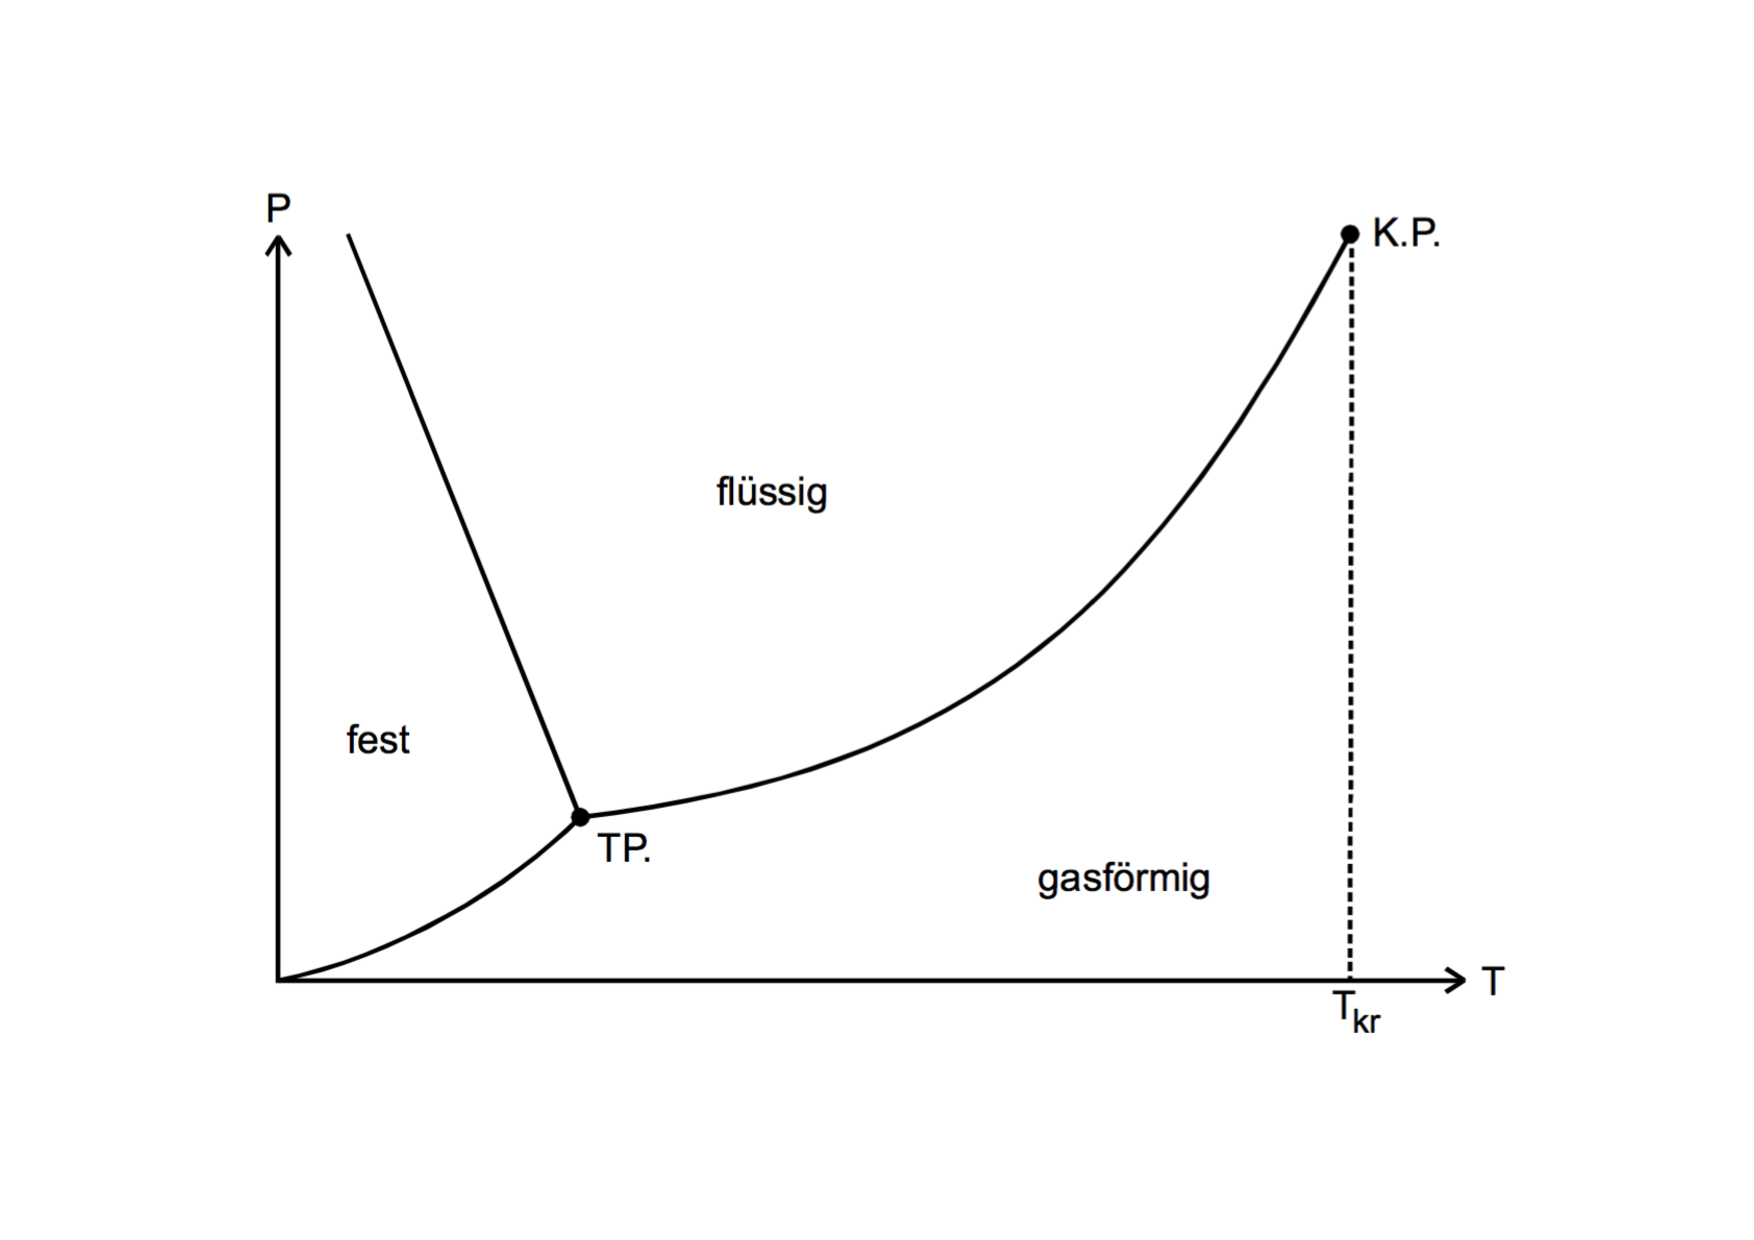
\includegraphics[height = 8cm]{Phasendiagramm.pdf}
  \caption{Qualitatives Zustandsdiagramm des Wassers.}
  \label{fig: Wasserdiagramm}
\end{figure}

In Abbildung \ref{fig: Wasserdiagramm} ist der Druck gegen die Temperatur aufgetragen.
Hier erkennt man, dass Kurven und auch Punkte existieren in deren unmittelbarer Umgebung zwei oder auch drei, wie beim Punkt TP, Phasen koexistieren können.

Im Folgenden wollen wir die Dampfdruckkurve untersuchen. Sie wird von den, in Abbildung \ref{fig: Wasserdiagramm} erkennbaren Punkten TP und KP
begrenzt. Wenn man sich auf ihr befindet tritt das Wasser in zwei Phasen auf: Flüssig und Gasförmig. Außerdem ist auf der $p(T)$-Kurve nur ein Freiheitsgrad
vorhanden, da zu jeder Temperatur ein Druck zugeordnet ist und andersherum.

Damit eine Gas-Phase entstehen kann, müssen zunächst einige Wassermoleküle aus der flüssigen Phase austreten. Hierfür benötigen sie zusätzliche
kinetische Energie. Wir führen den Begriff der Verdampfungswärme L ein. Sie bestimmt auch den Verlauf der Dampfdruckkurve. L ist
strenggenommen Temperaturabhängig, wie wir in Kapitel \ref{sec: MmA2} noch sehen werden. In dem Temperaturbereich in dem die Messwerte augenommen werden
aber ist die Verdampfungswärme fast konstant.

Wenn wir sie darauf beziehen, wie viel Energie ein Mol Wasser für den Phasenübergang von Flüssig zu Gasförmig benötigt ohne seine Temperatur zu
erhöhen, kommen wir auf den Begriff der molaren Verdampfungswärme $L_{m}$.

Bei Erhöhung der Temperatur erhalten die Wassermoleküle im System zusätzliche Energie und können in die Gas-Phase übertreten. Je mehr Wassermoleküle
in dieser Form vorliegen, desto höher steigt der Druck.
\newpage

\section{Aufbau}
\subsection{Apparatur 1}

  \begin{figure}[h!]
    \centering
    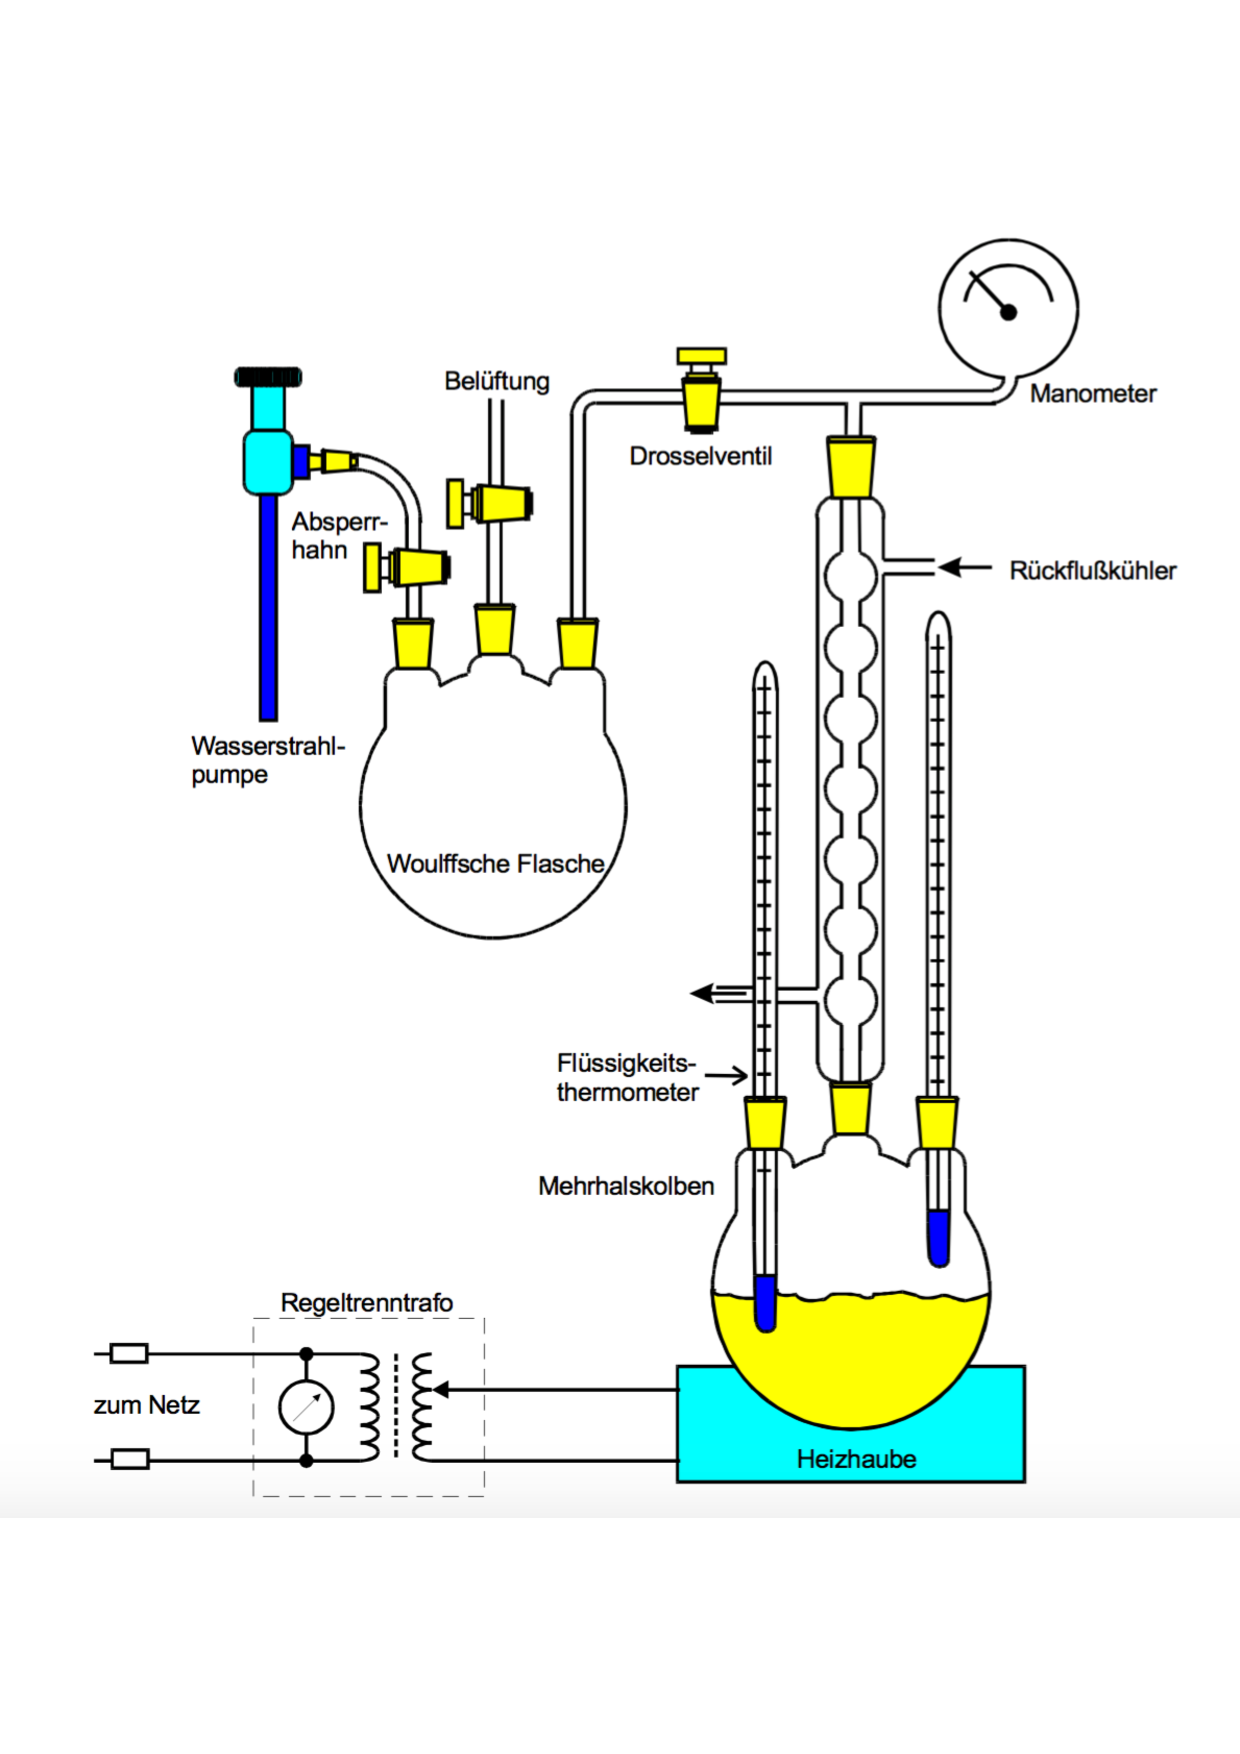
\includegraphics[height = 15cm]{Apparatur1.pdf}
    \caption{Apparatur 1 für den Druckbereich $p < 1$ \si{bar}.}
    \label{fig: Apparatur1}
  \end{figure}

\FloatBarrier

In Abbildung \ref{fig: Apparatur1} ist der Aufbau zur Bestimmung der Verdampfungswärme zu sehen.
Das Wasser wird mit Hilfe einer Heizhaube in einem evakuierten System, durch eine Wasserstrahlpumpe
realisiert, erhitzt. Die Temperatur kann
an zwei Thermometern abgelesen werden. Wobei eins in die Flüssigkeit reicht und das Andere in der
Gas-Phase misst. Der Druck wurde, anders als in der Abbildung, mit einem digitalen Messgerät gemessen.

\newpage

\subsection{Apparatur 2}

  \begin{figure}[h!]
    \centering
    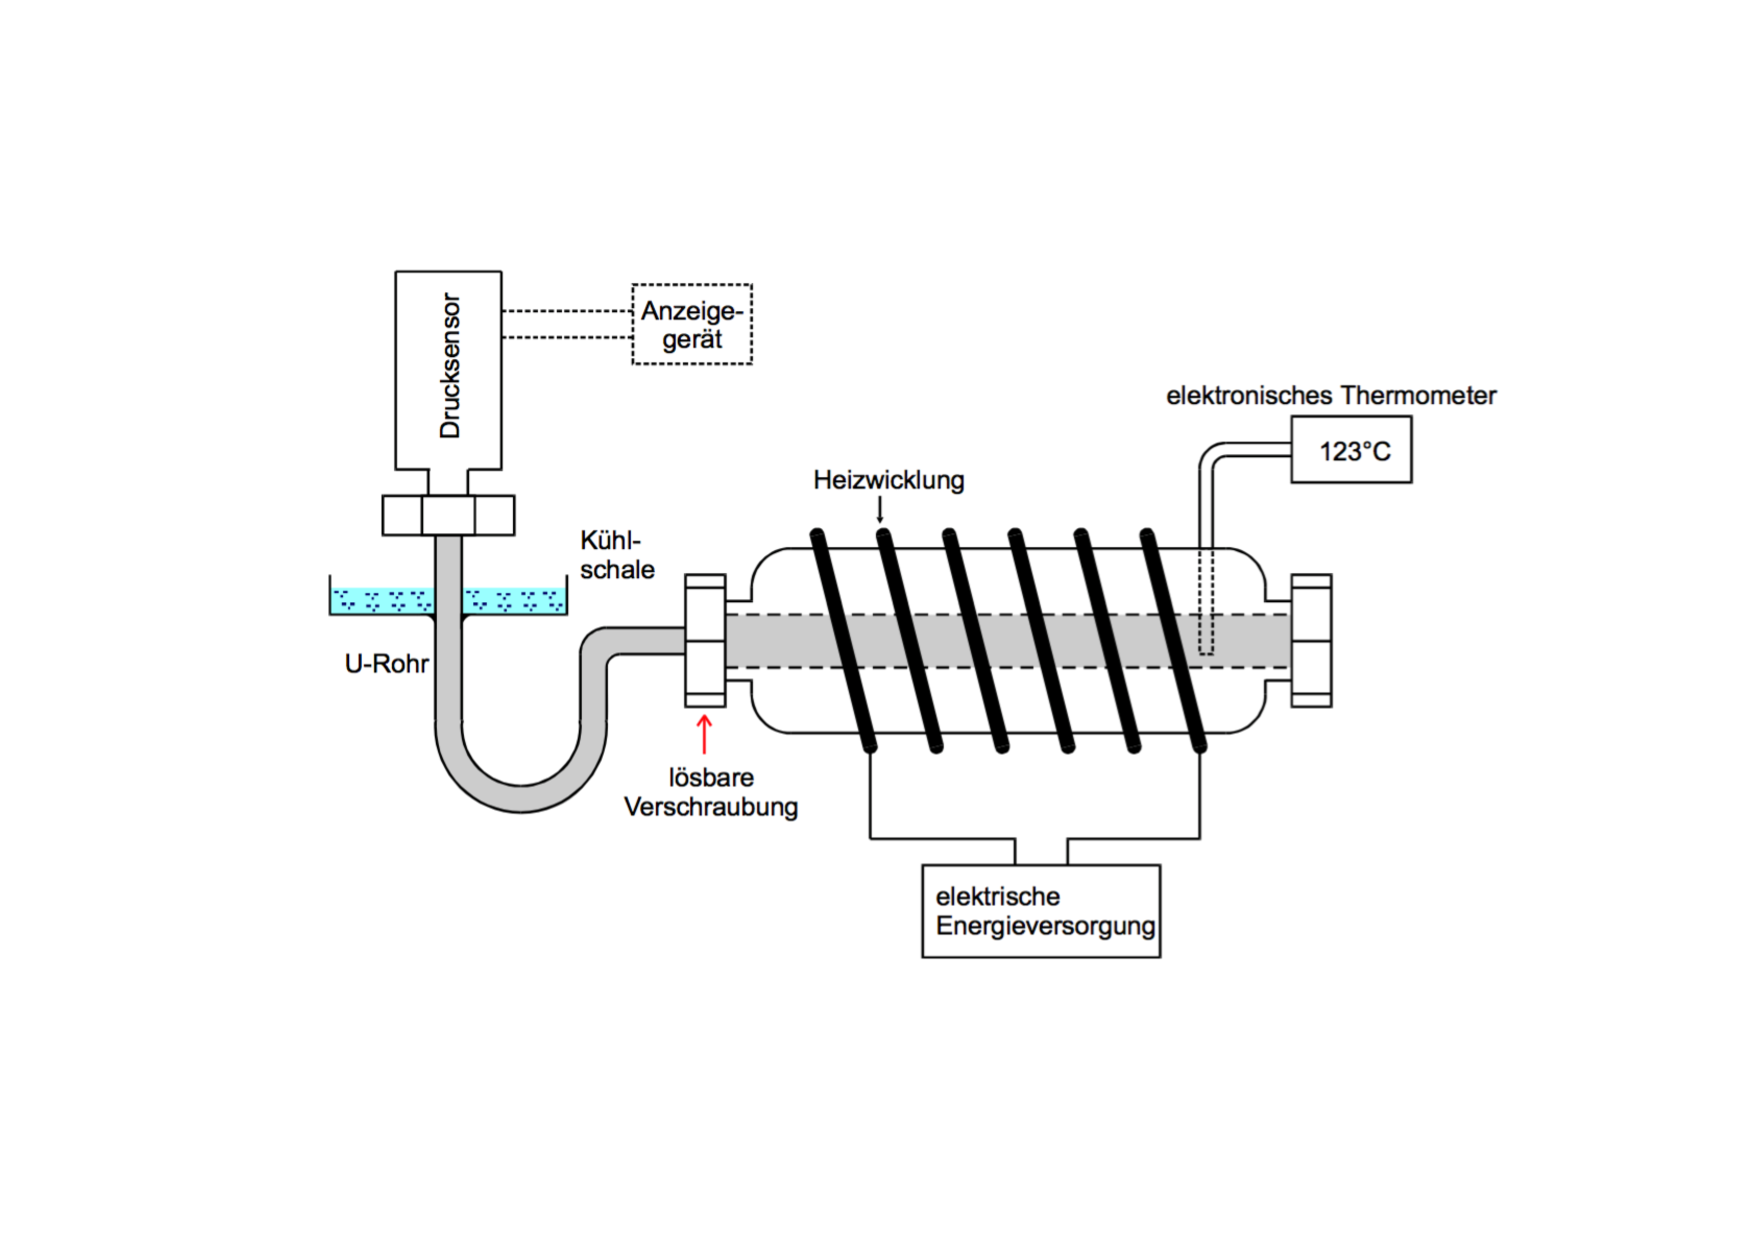
\includegraphics[height = 15cm]{Apparatur2.pdf}
    \caption{Apparatur 2 für den Druckbereich $p > 1$ \si{bar}.}
    \label{fig: Apparatur2}
  \end{figure}

\FloatBarrier

In Abbildung \ref{fig: Apparatur2} wird der Aufbau zur Messung des Drucks, in Abhängigkeit der
Temperatur, bei Werten $p > 1$ \si{bar} skizziert. Hier wurde Wasser in einem Behälter durch eine
Heizwicklung erhitzt und der Druck mit einem Drucksensor abgelesen. Ein elektronisches Thermometer
zeigt die Temperatur an.

\newpage

\section{Durchführung}
\label{sec:Durchführung}

\subsection{Apparatur 1}

Hier haben wir zunächst mit der Wasserstrahlpumpe den Druck im Innern des Sytems, so weit es möglich war,
gesenkt. Hierzu mussten die Ventile so geöffnet sein, dass es eine Verbindung zwischen der Pumpe
und dem Sytem gab. Nach Erreichen eines genügend kleinen Drucks wurden die Ventile geschlossen und
das Sytems so isoliert, dass der Druck weitestgehend konstant belibt.

Dann wurde die Heizhaube angeschaltet und zeitgleich die Durchlaufkühlung gestartet. Sobald das Wasser
siedete haben wir alle \SI{5}{\celsius} den Druck abgelesen bis zu einer Temperatur von \SI{100}{\celsius}.
Im Verlauf der Messung wurde die Kühlung immer weiter zurückgeschraubt bis sie zum Ende nur tropfenweise
lief.

\subsection{Apparatur 2}

Bei diesem Teil des Versuchs wurde zunächst der Offset bei \SI{100}{\celsius} gemessen. Dann haben wir bei
langsamem Anstieg der Temperatur alle \SI{3}{\celsius} den Druck abgelesen. Diese Messung lief bis \SI{127}{\celsius}.

\newpage


  \section{Auswertung}
  \subsection{Messergebnisse}
  \begin{table}[h]
    \centering
    \caption{Messdaten für Temperatur und Druck}
    \label{tab:a}
    \begin{tabular}{S S S S}
      \toprule
      \multicolumn{2}{c}{Druck < 1 bar} & \multicolumn{2}{c}{Druck > 1 bar} \\
      {$T/\si{\celsius}$} & {$p/\si{\milli\bar}$} & {$T/\si{\celsius}$} & {$p/\si{\bar}$} \\
      \midrule
      45 & 147 & 103 & 1.13 \\
      50 & 164 & 106 & 1.27 \\
      55 & 186 & 109 & 1.43 \\
      60 & 212 & 112 & 1.60 \\
      65 & 250 & 115 & 1.79 \\
      70 & 311 & 118 & 2.00 \\
      75 & 383 & 121 & 2.22 \\
      80 & 475 & 124 & 2.47 \\
      85 & 582 & 127 & 2.74 \\
      90 & 698 &  &  \\
      95 & 852 &  &  \\
      100 & 1011 &  &  \\
      \bottomrule
    \end{tabular}
  \end{table}
  Auf der linken Tabellenhälfte \ref{tab:a} sind die Messwerte für Druck
  ($p < 1$\si{bar}) und Temperatur aufgezeichnet,
  die mit Apparatur 1(siehe Abbildung \ref{fig: Apparatur1}) aufgenommen wurden. Auf der rechten Hälfte sind die
  Messwerte, die mit Apparatur 2(siehe Abbildung \ref{fig: Apparatur2}) aufgenommen wurden,
  allerdings wurde hier der Offset-Druck bereits mit eingerechnet. \\ \\
  Offsetdruck für die zweite Messung ($p > 1\si{bar}$):
  \begin{equation}
    p_\text{offset} = 0.2 bar
  \end{equation}

  \subsection{Graphen und Rechnung}
  \subsubsection{Messung mit Apparatur 1}
  In dem Graphen \ref{fig:p1(T)} ($p < 1$\si{bar})
  ist der Logarithmus des Dampfdruckes $p$ (in \si{\kPa})
  gegen die reziproke absolute Temperatur (in \si{\kelvin}) dargestellt.
  Mit der Funktion linregress aus scipy.stats
  wurde eine Ausgleichsgerade erstellt, für die folgende Werte für den
  Y-Achsen-Abschnitt $b$ und die Steigung $m$ zurückgegeben wurden (umgerechnet
  von \si{\kPa} in \si{\Pa}):
  \begin{equation}
    p_1(T) = m \cdot T + b
  \end{equation}
  \begin{align}
    b & = 29.998 &  m & = \num{-4344.8 +- 169.3}
  \end{align}
  \begin{figure}
    \centering
    \includegraphics[height = 8.30 cm]{plot.pdf}
    \caption{Messwerte von Apparatur 1, Graph p1(T)}
    \label{fig:p1(T)}
  \end{figure}

  Die gemittelte Verdampfungswärme $L$ pro \si{mol} für den Druckbereich
  $p < 1\si{bar}$ lautet nun
  \begin{equation}
    L = -m \cdot R \cdot \si{\kelvin} =
    \SI{36122.6672 +- 1407.5602}{\joule\per\mol}
  \end{equation}
  mit der allgemeinen Gaskonstante\cite{gaskonstante}
  $R = 8.314\si[per-mode=reciprocal]{\joule\per\kelvin\per\mol}$.
  Die äußere Verdampfungswärme $L_a$ pro \si{mol} bei $T = 373\si{\kelvin}$ ist
  \begin{equation}
    L_a = T \cdot R = 3101.122 \si{\joule\per\mol}.
  \end{equation}
  Aus diesen Werten ergibt sich dann die innere Verdampfungswärme $L_i$, die
  zur Überwindung der molekularen Anziehungskräfte bei der Verdampfung benötigt
  wird:
  \begin{equation}
    L_i = L - L_a = \SI{2.0610428289(0878530014)e27}{\electronvolt\per\mol}
  \end{equation}
  Um die innere Verdampfungswärme pro Molekül zu bestimmten muss man noch durch
  die Avogadro-konstante\cite{avogadro}
  ($N_A = 6.022 \cdot 10^{23} \si[per-mode=reciprocal]{\per\mol}$) teilen:
  \begin{equation}
    L_{i,m} = \frac{L_i}{N_A} = \SI{3422.5221336 +- 145.8867509}{\electronvolt}
  \end{equation}
  \newpage
   \subsubsection{Messung mit Apparatur 2}
  \label{sec: MmA2}
  In dem Graphen \ref{fig:p2(T)} ($p > 1$\si{\bar}) ist der Dampfdruck
  $p$ (in \si{\kPa}) gegenüber der absoluten Temperatur $T$ (in \si{\kelvin})
  aufgetragen. Das Ausgleichspolynom dritten Grades wurde mit Hilfe der
  Funktion polyfit aus numpy erstellt.
  Dabei wurden folgende Werte für die Funktionsgleichung zurückgegeben
  (umgerechnet von \si{\kPa} in \si{\Pa}):
  \begin{equation}
    p_2(T) = aT³ + bT² + cT + d
  \end{equation}
  \begin{align}
    a & = 0.84 & b & = -880.01 \\
    c & = 309277.95 & d & = -36508852.61
  \end{align}
  \begin{figure}[h]
    \centering
    \includegraphics[height = 8.30 cm]{plot2.pdf}
    \caption{Messwerte von Apparatur 2, Graph p2(T)}
    \label{fig:p2(T)}
  \end{figure}
  \\
  Um eine Abhängigkeit zwischen der Verdampfungswärme $L$ und der Temperatur
  $T$ bei einem Druck $p > 1\si{\bar}$ herauszufinden löst man zunächst die
  Clausius-Clapeyronsche Gleichung nach $L$ auf.
  \begin{equation}
    (V_D - V_F) dp = \frac{L}{T} dT
    \iff L = (V_D - V_F) \frac{dp}{dT} T
  \end{equation}
  Nun ist der Differentialquotient $\frac{dp}{dT}$ die Ableitung der
  Ausgleichsfunktion $p_2(T)$:
  \begin{equation}
    p_2'(T) = 2.25 T² - 1760.02 T + 309277.95
  \end{equation}
  Das Flüssigkeits-Volumen $V_F$ pro Mol wird über die molare Masse und die
  Dichte von Wasser\cite{stoffwerte}
  (bei $T = 373 K$, $p = 100000 \si{\Pa}$) berechnet:
  \begin{align}
    M_W & = \underbrace{2 \cdot 1}_{H_2} + \underbrace{16}_{O}
    \si{\gram\per\mol} & \rho_W & = 950000 \si{\gram\per\cubic\meter}
  \end{align}
  \begin{equation}
    V_F = \frac{M_W}{\rho_W} = 1.894736 \cdot 10^{-5} \si{\cubic\meter\per\mol}
  \end{equation}
  Das Dampf-Volumen $V_D$ pro Mol kann über die folgende Gleichung genähert
  werden:
  \begin{equation}
    \Bigl(p + \frac{a}{V²}\Bigr)V = R T
  \end{equation} mit $T = 373 \si{\kelvin}$, $p = 100000 \si{\Pa}$ und
  $a = 0.9 \si[per-mode=reciprocal]{\joule\cubic\meter\per\mol\squared}$.
  Durch umformen mit der \\
  pq-Formel erhält man dann einen sinnvollen Wert
  \begin{equation}
    V_D = 0.03072569441 \si{\cubic\meter\per\mol}
  \end{equation} für das Dampfvolumen.
  Zuletzt setzt man die Werte in die umgeformte
  Clausius-Clapeyronsche Gleichung ein und erhält für die Verdampfungswärme in
  Abhängigkeit von der Temperatur folgende Funktion:
  \begin{equation}
    L(T) = 0.691 \cdot T³ + 54.044 \cdot T² + 9499.919 \cdot T
  \end{equation}
  \newpage
  \subsection{Diskussion der Ergebnisse}
  In Abbildung \ref{fig:p1(T)} kann man erkennen, dass die Messwerte sehr nah
  an der durch die Funktion linregress bestimmten Geraden liegen. Der $r$-Wert
  (r = 0.9924) bestätigt die Annahme, dass die Verdampfungswärme von Wasser im
  Druckbereich $p < 1 \si{\bar}$ annähernd konstant ist. Auffällig ist, dass
  die berechnete äußere Verdampfungswärme $L_a$, die zur Volumenausdehnung (und
  damit zur Druckerhöhung im Gefäß) nötig ist, deutlich kleiner als die innere
  Verdampfungswärme $L_i$, die zur Überwindung der molekularen Anziehungskräfte
  benötigt wird, ist ($L_i > 10 \cdot L_a$).
  Das liegt daran, dass $L_i$ die kinetische Energie $E_\text{kin}$ der Moleküle in
  der Flüssigkeit so erhöhen muss, dass der Anteil mit maximaler kinetischer
  Energie (Maxwellsche Geschwindigkeitsverteilung) wächst.
  Die äußere Verdampfungswärme $L_a$ sorgt lediglich dafür, dass die Moleküle
  im Wasserdampf, die deutlich weniger gebunden sind und mehr Platz haben,
  zusammengedrückt werden ($V = const, p > p_0$).

  In Abbildung \ref{fig:p2(T)} erkennt man, dass Druck und Temperatur ab
  $p > 1\si{\bar}$ anders voneinander abhängen und die latente Wärme $L$
  dadurch nicht mehr als konstant angesehen werden kann. Ein Polynom dritten
  Grades kommt den Messwerten von Druck und temperatur sehr nahe.
  Bei der berechneten Verdampfungswärme $L(T)$ muss man beachten, dass in der zur
  Berechnung benutzten Formel Drücke und Volumina als konstant
  angenommen wurden, was nur stark genähert zutrifft. Den Graphen von $L$ sieht
  man in Abbildung \ref{fig:L}.
  \begin{figure}[h]
    \centering
    \includegraphics[height = 8.30 cm]{plot3.pdf}
    \caption{Verdampfungswärme bei $p > 1\si{\bar}$, Graph $L(T)$}
    \label{fig:L}
  \end{figure}

  \newpage


\section{Anhang}
\subsection{Kopie der Originaldaten}
\newpage

\nocite{*}

\printbibliography

\end{document}
